% Compact layout of the original raster plots. Only margins and legends
% are replaced by vector annotations; plotted curves/bands are unchanged.
% Coordinates below refer to the 1189 x 690 source-image pixels.
\begin{figure*}[t]
\centering
\definecolor{stressavg}{HTML}{1F77B4}
\definecolor{stressprox}{HTML}{FF7F0E}
\definecolor{stressscaffold}{HTML}{2CA02C}
\definecolor{stressfused}{HTML}{D62728}
{\small
\textcolor{stressavg}{\rule[.5ex]{12pt}{1pt}}\,FedAvg\quad
\textcolor{stressprox}{\rule[.5ex]{12pt}{1pt}}\,FedProx\quad
\textcolor{stressscaffold}{\rule[.5ex]{12pt}{1pt}}\,SCAFFOLD\quad
\textcolor{stressfused}{\rule[.5ex]{12pt}{1pt}}\,FusedSpaceFed
\par}\smallskip
\begin{tikzpicture}[x=.183pt,y=.183pt,every node/.style={font=\scriptsize,text=black}]
  \begin{scope}
    \clip (0,0) rectangle (1105,597);
    \node[anchor=south west,inner sep=0] at (-67,-58)
      {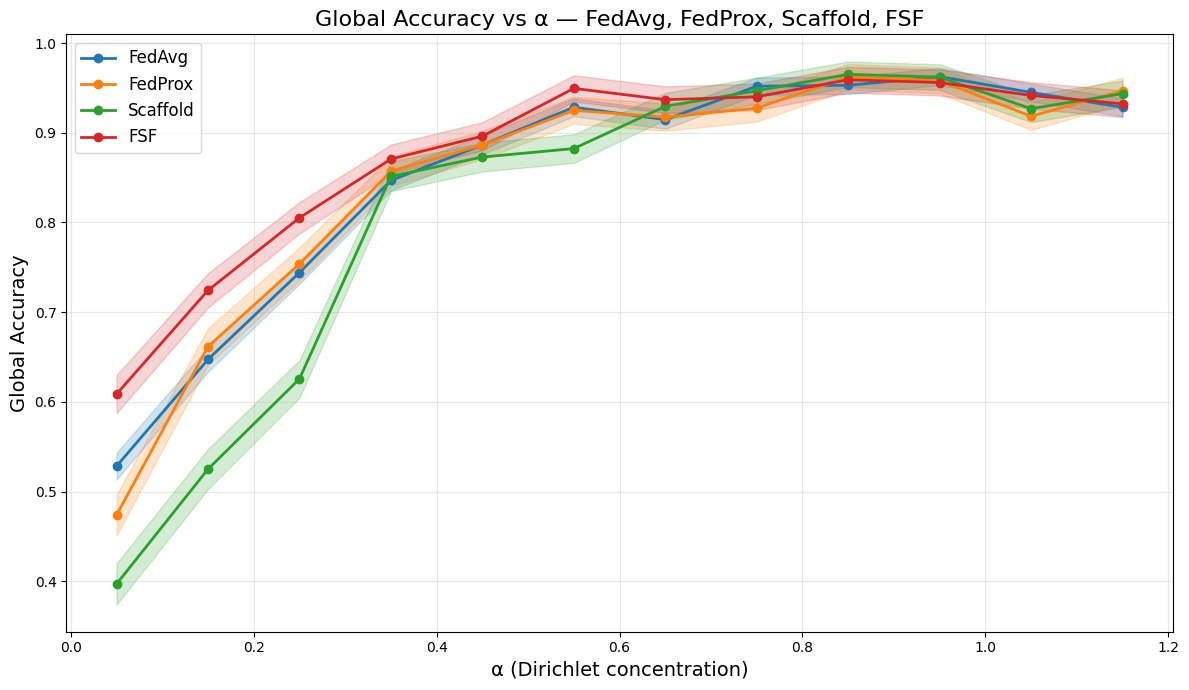
\includegraphics[width=217.587pt]{accuracy_FSF.jpg}};
    % Mask the existing opaque legend box, not the plotted data.
    \fill[white] (8,478) rectangle (136,589);
  \end{scope}
  \draw[black,line width=.25pt] (0,0) rectangle (1105,597);
  \foreach \x/\value in {4/0.0,187/0.2,370/0.4,553/0.6,735/0.8,918/1.0,1101/1.2}{
    \draw[black,line width=.25pt] (\x,0)--(\x,-9);
    \node[anchor=north] at (\x,-11) {\value};
  }
  \foreach \y/\value in {51/0.4,140/0.5,230/0.6,320/0.7,410/0.8,499/0.9,589/1.0}{
    \draw[black,line width=.25pt] (0,\y)--(-9,\y);
    \node[anchor=east] at (-11,\y) {\value};
  }
  \node at (552,636) {\textbf{(a)} Test accuracy};
  \node at (552,-95) {Dirichlet concentration $\alpha$};
\end{tikzpicture}
\hfill
\begin{tikzpicture}[x=.183pt,y=.183pt,every node/.style={font=\scriptsize,text=black}]
  \begin{scope}
    \clip (0,0) rectangle (1111,598);
    \node[anchor=south west,inner sep=0] at (-62,-58)
      {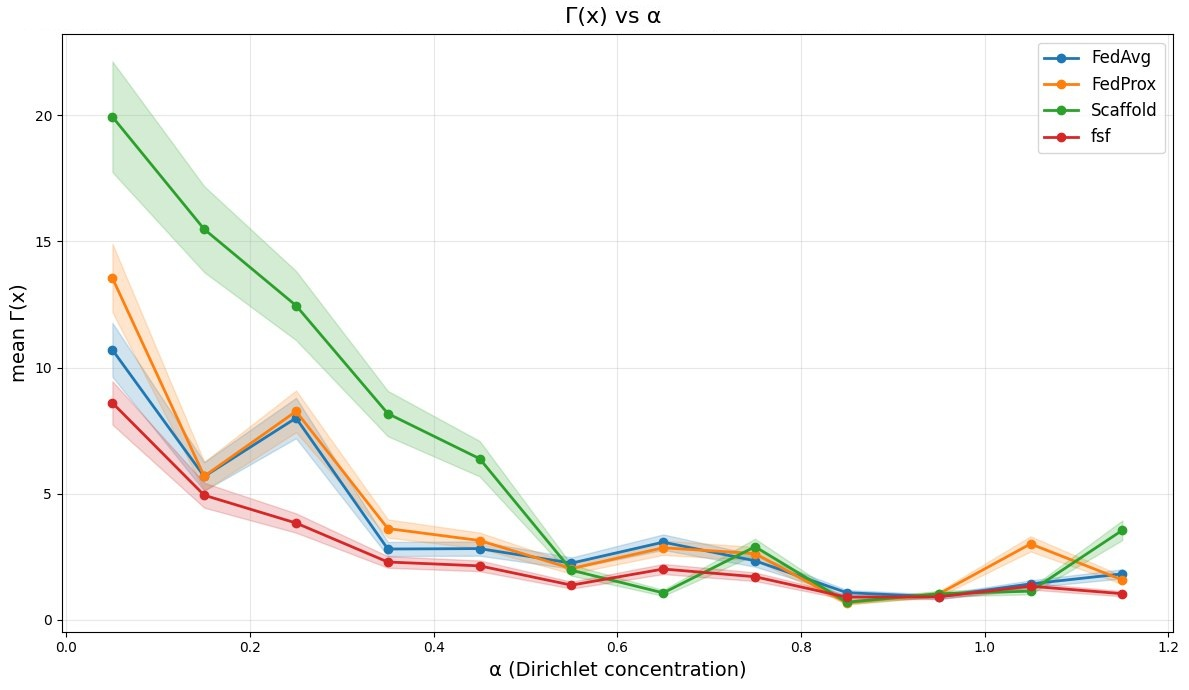
\includegraphics[width=217.587pt]{gamma_FSF.jpg}};
    % The covered region is the original opaque legend.
    \fill[white] (976,478) rectangle (1102,589);
  \end{scope}
  \draw[black,line width=.25pt] (0,0) rectangle (1111,598);
  \foreach \x/\value in {4/0.0,188/0.2,372/0.4,555/0.6,739/0.8,923/1.0,1106/1.2}{
    \draw[black,line width=.25pt] (\x,0)--(\x,-9);
    \node[anchor=north] at (\x,-11) {\value};
  }
  \foreach \y/\value in {12/0,138/5,264/10,391/15,517/20}{
    \draw[black,line width=.25pt] (0,\y)--(-9,\y);
    \node[anchor=east] at (-11,\y) {\value};
  }
  \node at (555,636) {\textbf{(b)} Classifier-gradient dispersion $\Gamma_t$};
  \node at (555,-95) {Dirichlet concentration $\alpha$};
\end{tikzpicture}
\caption{PathMNIST stress test: (a) test accuracy and (b) final-round
classifier-gradient dispersion $\Gamma_t$ from
Equation~\eqref{eq:gradient_dissimilarity}, versus Dirichlet concentration
$\alpha$. Dots indicate means across five independent runs; shaded areas
show the corresponding standard deviations.}
\label{fig:pathmnist_stress}
\end{figure*}
